% 05.04.2024
\section{Dynamic Graphs, Lecture 7}

Online algorithms for dynamic graphs.

\begin{df}
  We would have stream with three type of queries:
  \begin{enumerate}
	  \item insert
	\item delete
	\item query
  \end{enumerate}

  We would have such types of analysis:

  \begin{enumerate}
	  \item worst-case / ammortize
	\item  deterministic / random
	\item oblivious / nonoblivious (can the stream depends on our answers/memory/randomness?)
  \end{enumerate}

  So, the base case is when our analysis is worst-case deterministic.
\end{df}

\begin{df}[Connectivity problem] \label{df:connectivity}
	Allow insert edge $e$, delete edge $e$ and query: is it possible to reach $j$ from $i$? 
\end{df}

\begin{thm}
	Directed connectivity problem \ref{df:connectivity} is SETH-hard(for any strongly sublinear time), in case when query is asking how many vertices is reachable from $i$.
\end{thm}

\begin{proof}
  From $k$-SAT we construct a graph as follows:

\begin{figure}[H]
	\centering
	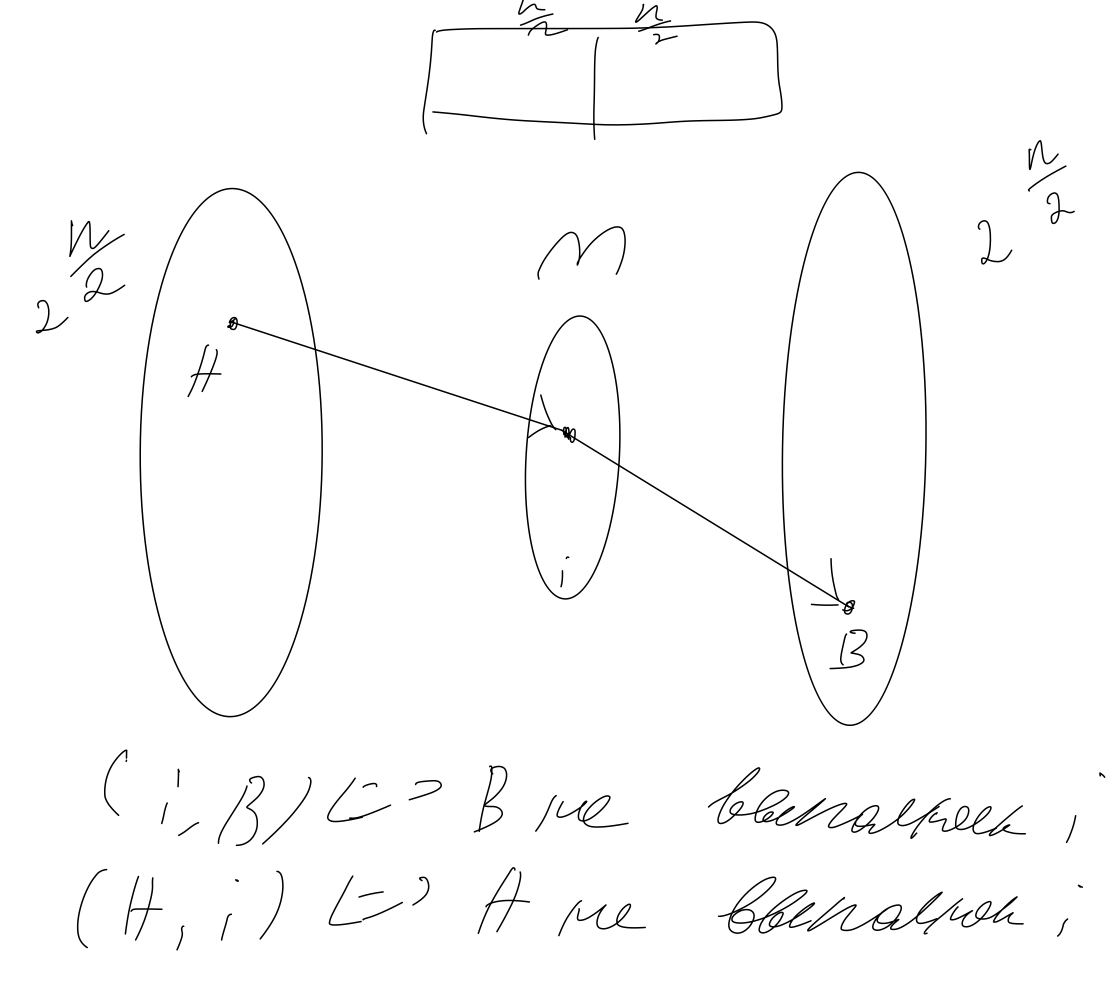
\includegraphics[width=0.5\linewidth]{figures/connectivity_seth_hard.jpeg}
	\caption{Reduction from $k$-SAT to Connectivity.}
	\label{fig:connectivity_seth_hard}
\end{figure}

  Size of left part is $2^{\frac{n}{2}}$, middle is $m$ and right is also $2^{\frac{n}{2}}$, where $n$ is a number of variables, $m$ is a number of clauses. And each vertex in the most left part encodes first $\frac{n}{2}$ variables, the most right parts encodes values of last $\frac{n}{2}$ variables.

  So, if we find a pair of vertices $A, B$ such that there is no path from $A$ to $B$, if and only if instance is SAT.
\end{proof}

For now consider insert/delete operations, we would maintain forest of spanning trees(collection of spanning trees for every connected component).
Later we would see what queries we can do on that spanning forest.

\begin{algorithm}[Freckerson?]
  There exists an algorithm with update time would be $m^{\frac{2}{3}}$, where $m$ is a current amount of edges in graph.
\end{algorithm}

\begin{proof}
  Assume current spanning forest.

  We would store not just a forest, but also partition of our forest into connected blocks, each block $T$ would be the size between $z \leq |T| \leq 3 z$(except trees of small size) for some parameter $z$. See Fig. \ref{fig:connectivity_m_2_3_blocks}.

\begin{figure}[H]
	\centering
	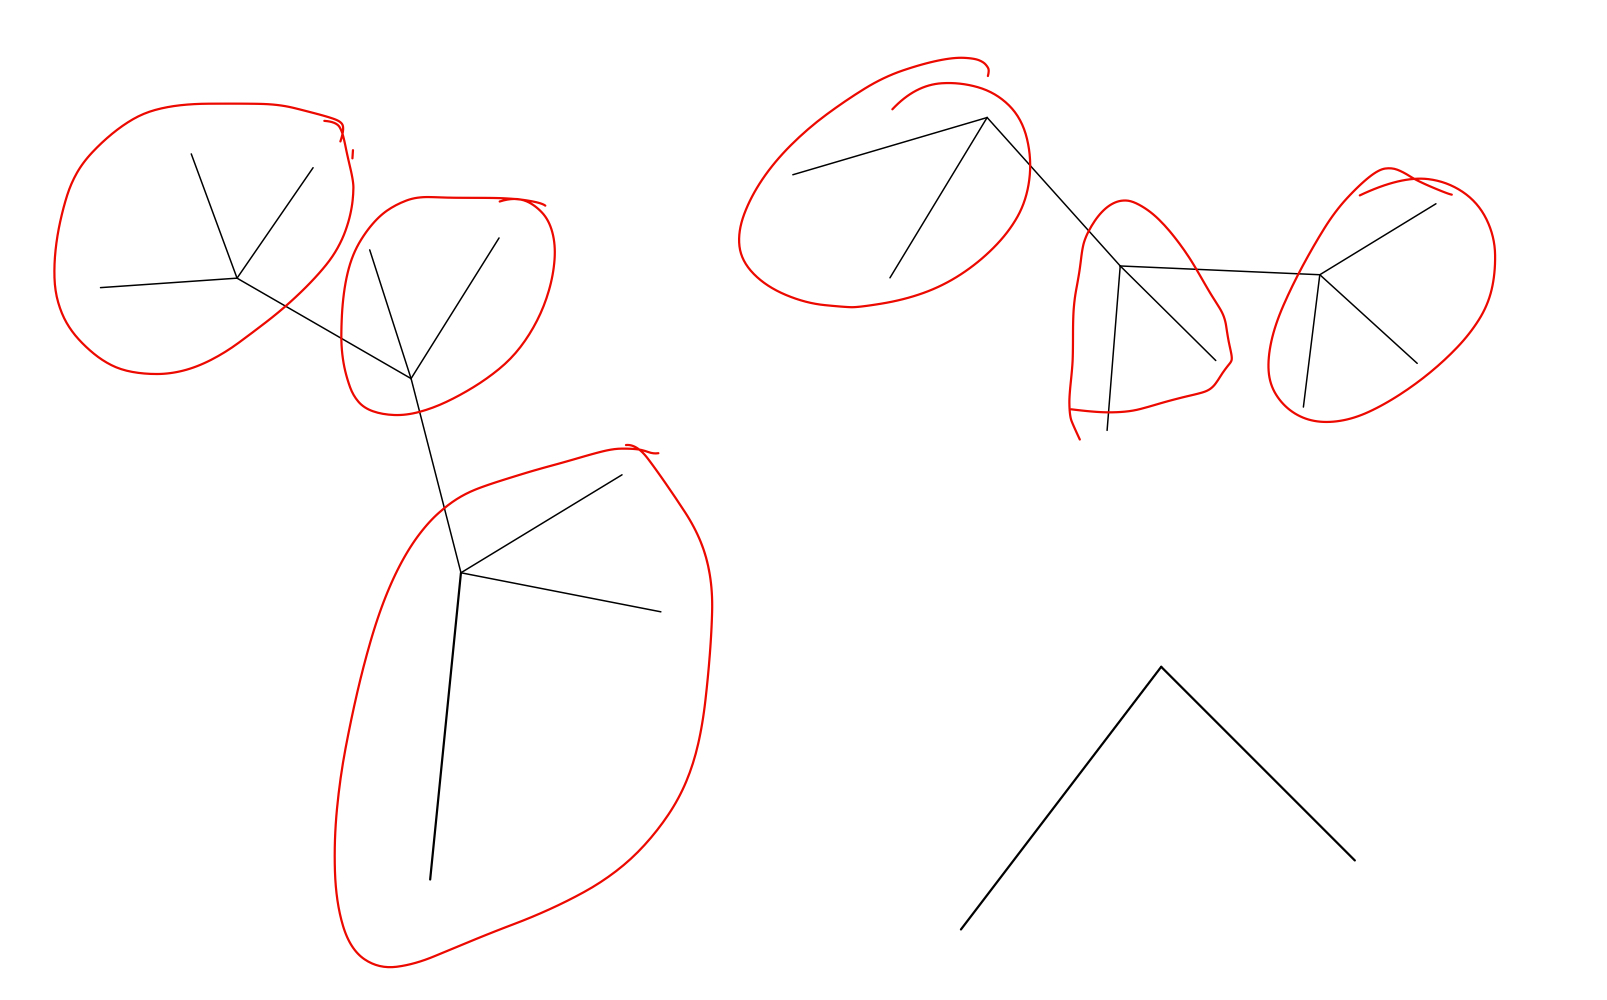
\includegraphics[width=0.5\linewidth]{figures/connectivity_m_2_3_blocks.jpeg}
	\caption{Splitting forest into blocks.}
	\label{fig:connectivity_m_2_3_blocks}
\end{figure}

First of all we assume that our tree is binary, we can do it by following operation, assume vertex of degree more than 3, we would convert it to cycle and add some new edges, Fig. \ref{fig:connectivity_degree_3}.


\begin{figure}[H]
	\centering
	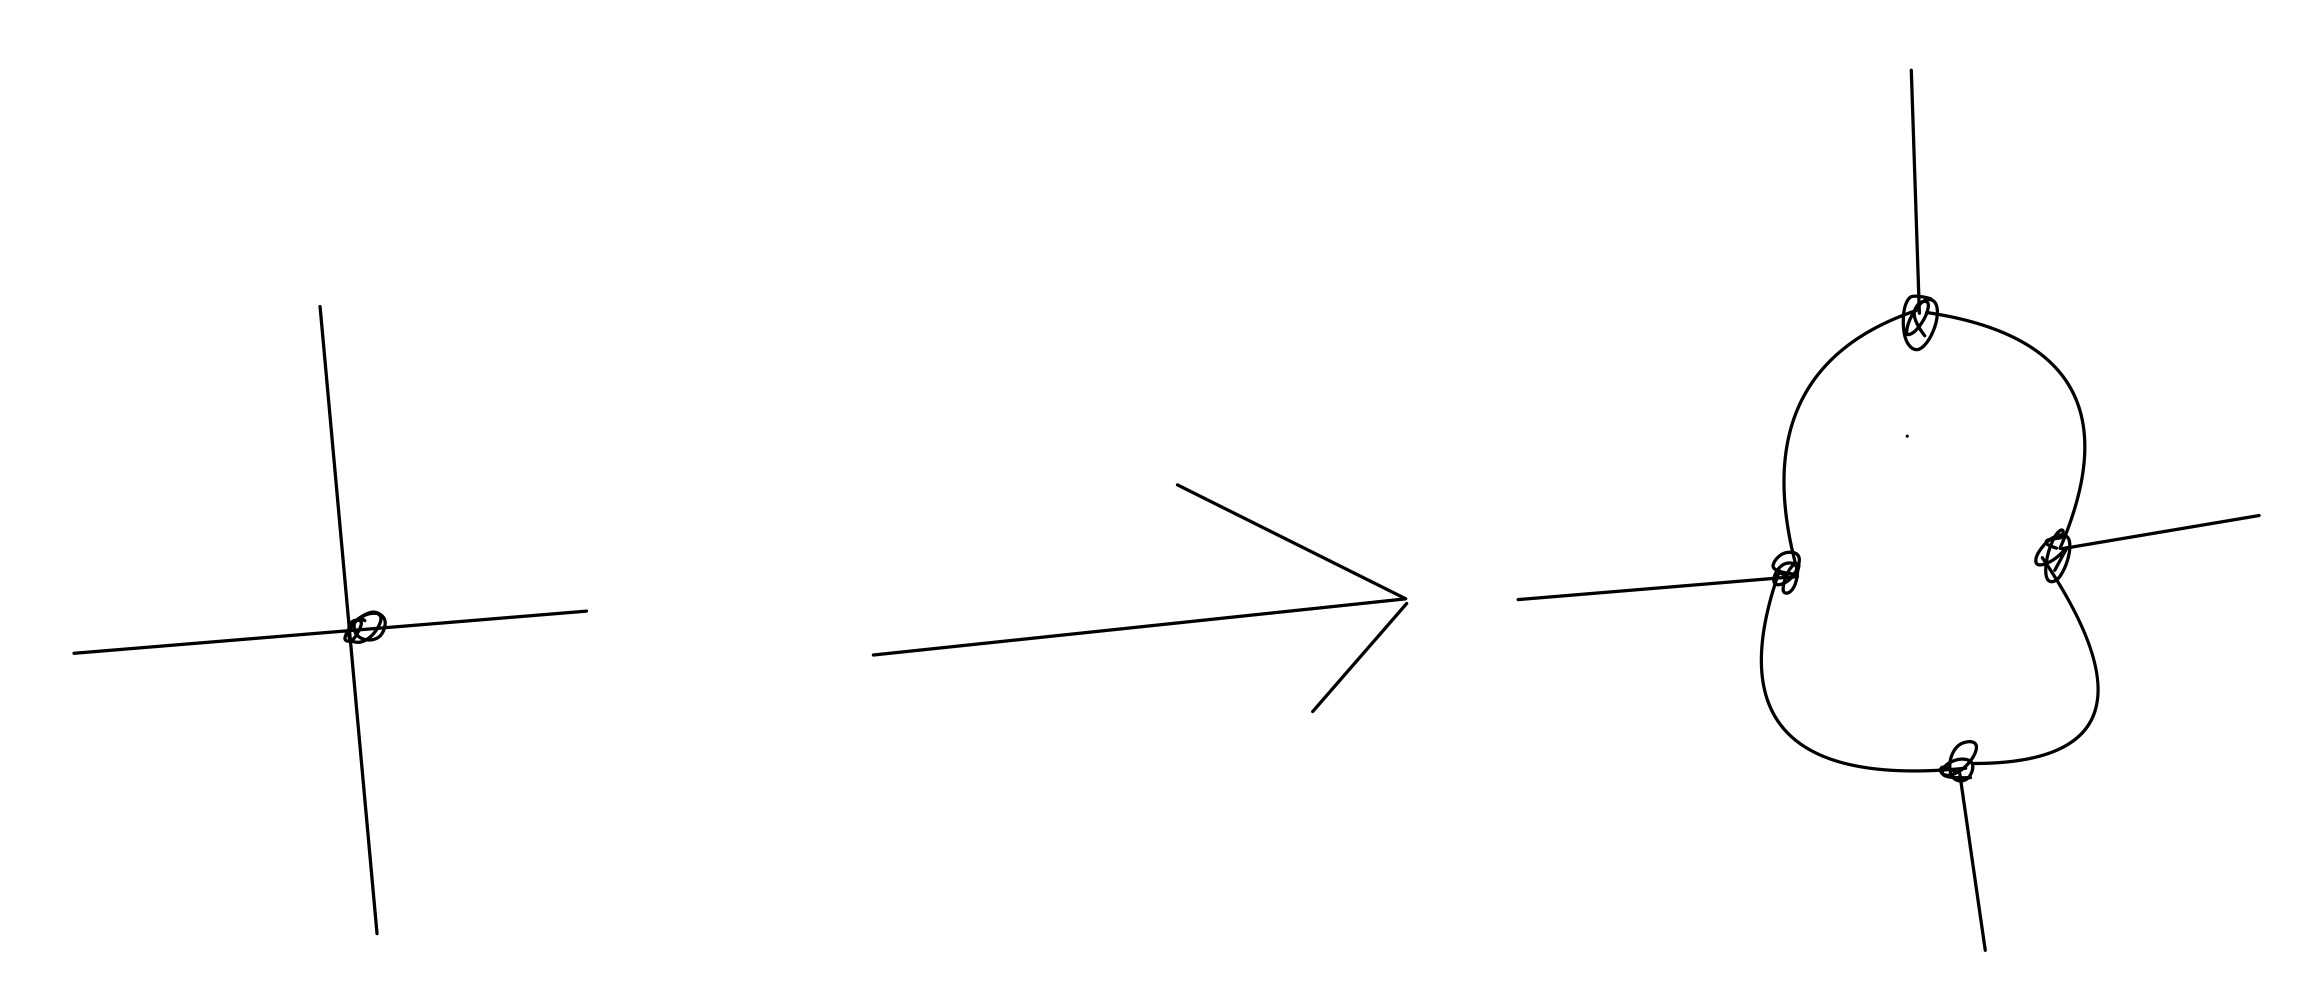
\includegraphics[width=0.5\linewidth]{figures/connectivity_degree_3.jpeg}
	\caption{Making degree of each vertex at most 3.}
	\label{fig:connectivity_degree_3}
\end{figure}

After such operation our amount of vertices is roughly amount of edges, i.e. $m$.

  It's possible because in any tree $T$ there exists subtree $T_i$ such that $\frac{|T|}{3} \leq |T_i| \leq \frac{2|T|}{3}$, because we can always go to the biggest child and it some point it would satisfy this property. So after we just separately split into blocks $T_i$ and $T \setminus T_i$.

  And for each pair of blocks we contain a list of edges between them (green on a picture \ref{fig:connectivity_removing_edge})

\begin{figure}[H]
	\centering
	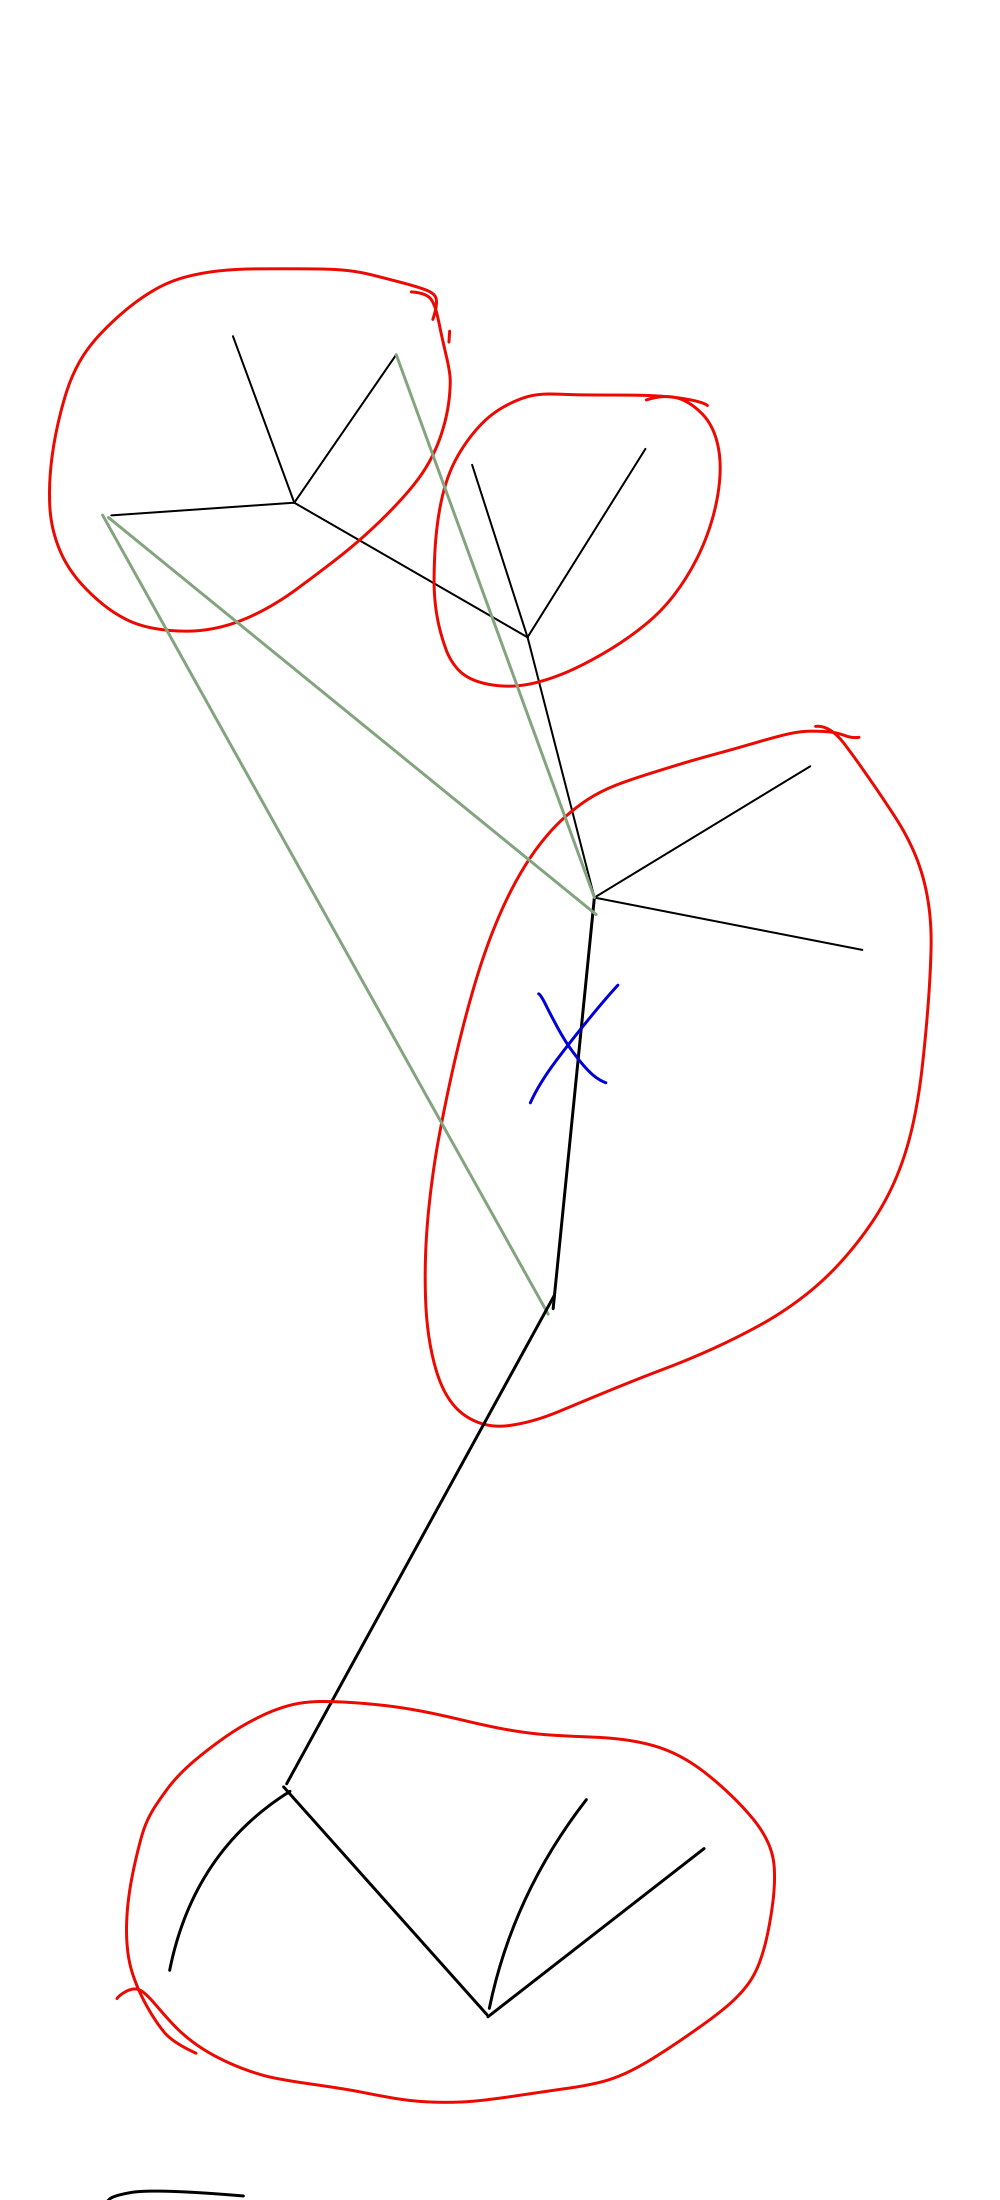
\includegraphics[width=0.25\linewidth]{figures/connectivity_removing_edge.jpeg}
	\caption{Removing edge.}
	\label{fig:connectivity_removing_edge}
\end{figure}

  Having such construction, to add new edge we do the following:

  \begin{itemize}
	  \item if edge connecting vertices from different trees, then we add new "black" edge(making it an edge of the forest), and that's all. Maybe this tree won't be small and we would split it into blocks. If those trees is large, then $O(1)$, if resulting is large, then we would spend reconstructing time(to be specified later).
	\item If an edge is inside of a block, than nothing happens. $O(1)$.
	\item And if an edge is between different blocks of one tree, then we should just add edge to a list of those blocks. $O(1)$.
  \end{itemize}

  On delete:

  \begin{itemize}
	  \item If we deleting an edge and spanning trees does not change, then we just remove it from a list of two blocks.
	  \item If an edge is inside a block, then we check blocks connectivity using $O(z)$ time(because each tree is of degree 3). If we cannot find alternative, we firstly check it our entire tree is connected in time $O(z) + O(\frac{m^2}{z^2})$, we check every pair of blocks from left side and right side. After that we may need rebalancing of our tree.
	\item If we delete edge between two different trees, then it's the same as previous point, but we do not spend $O(z)$ time.
  \end{itemize}

  Rebalancing:
  We need to rebalance one small block. We would merge this small block and two it's adjacent.
  Using $O(z)$ time to find two adjacent blocks and $O(z)$ for lists constructing, using fact that degree of every vertex is no more than $3$.

\begin{figure}[H]
	\centering
	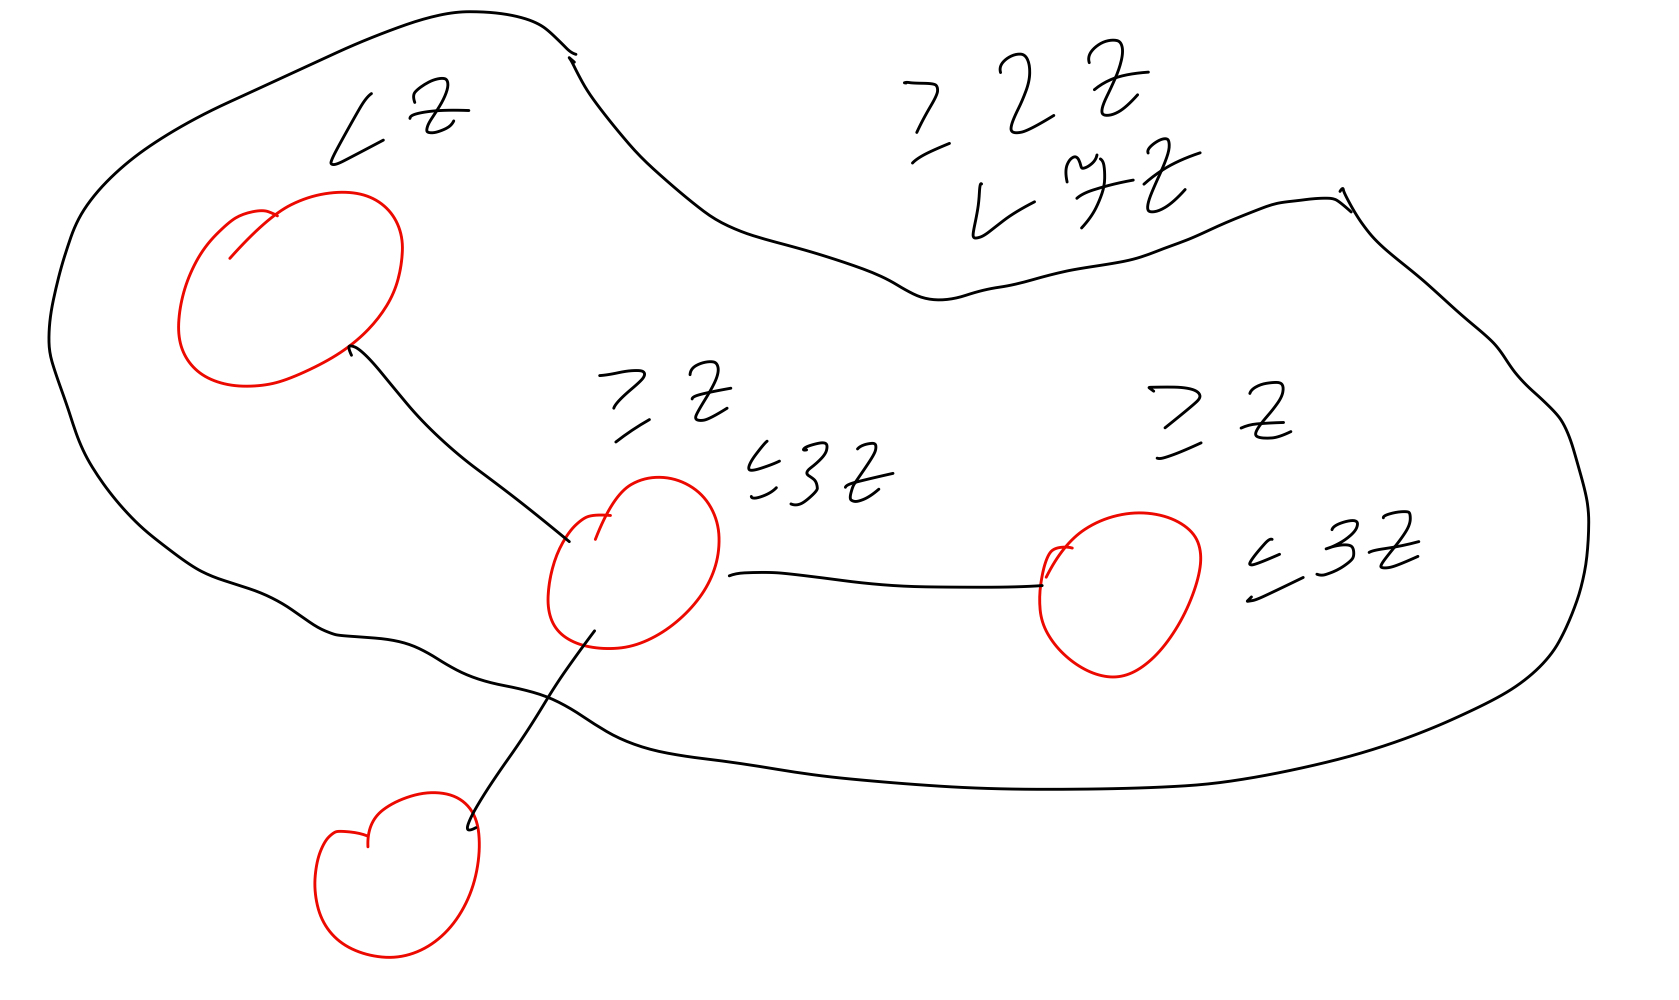
\includegraphics[width=0.5\linewidth]{figures/connectivity_rebalancing.jpeg}
	\caption{Rebalancing forest.}
	\label{fig:connectivity_rebalancing}
\end{figure}

  After that substituting $z = m^{\frac{2}{3}}$ we get needed time.

\end{proof}

\begin{algorithm}
	There exists an amortized algorithm with update time would be $\log^{O(1)} m$, where $m$ is a current amount of edges in graph.
\end{algorithm}

Whenever an edge is added, we have a bunch of tokens on edge.
And those tokens are some function for estimating amortized time.

\begin{thm}
	Connectivity problem \ref{df:connectivity} can be solved in time $O(\log^2 n)$ amortized time on query.
\end{thm}

\begin{proof}
Idea is that every edge would have a level, some number $l(e) \in [0, \log n]$.

Those levels gives us a partition of a graph into subgraphs with edges with every level, we would note $G_0 = G$ and $V(G_i) = V(G)$ and $E(G_i) = \{ e \mid e \in E(G) \wedge l(e) \geq i\}$.

And let $F_i$ be a spanning forest of $G_i$.
And with property that they are nested, i.e. $F_i \subseteq F_{i - 1}$.

And additionally we would try to keep $F_i = G_i \cap F_0$.

To make it possible we would construct $F_0$ as max weight spanning forest where weight of an edge $e$ is $2^{l(e)}$ or $l(e)$(both works).

Whenever we are adding an edge we add it to lever $0$ and put $\log n$ tokens to this edge.
Whenever we are touching an edge(for whenever reason) we would raise it's level and reduce amount of tokens on it.
It means, that the number of times we've touched an edge is at most $m \log n$.

When we add an edge, see Fig. \ref{fig:connectivity_adding_edge_spanning}:
\begin{itemize}
	\item Level of new edge is $0$, so if it's inside single tree, we would do nothing.
	\item Otherwise, we just merge two different trees on zero level.
\end{itemize}

\begin{figure}[H]
	\centering
	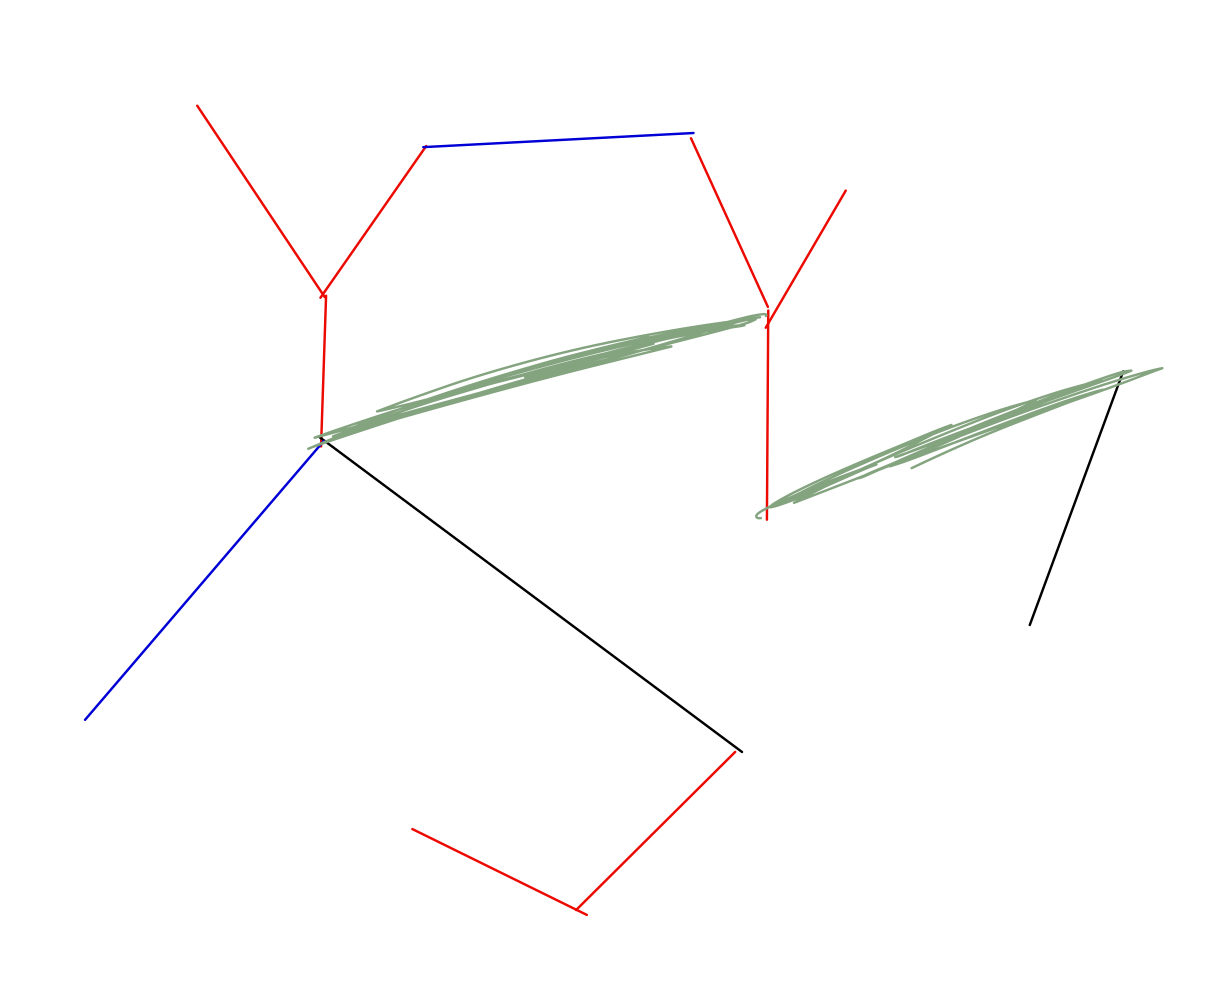
\includegraphics[width=0.5\linewidth]{figures/connectivity_adding_edge_spanning.jpeg}
	\caption{Adding an edge, black is edges of level 0, blue is of level 1, red is of level 2. Green edges is possible new edges.}
	\label{fig:connectivity_adding_edge_spanning}
\end{figure}

We would store our trees in ET-tree structure \ref{df:et_tree}, that allows to merge/split tree in $\log$ time.

if we delete an edge:
\begin{itemize}
	\item When we delete an edge, we need to find an alternative connecting edge. Level of new edge cannot be more than level of deleted edge, because otherwise we didn't construct a maximum spanning tree on top level.
	\item We would search for an alternative on it's level(green subspace on figure \ref{fig:connectivity_deleting_spanning}). 
\end{itemize}
Assume that level of deleted edge is $k$.
$T$ splitted into $T_1, T_2$, where $|T_1| \leq |T_2|$ and $\forall e \in T_1 \mid l(e) = k \implies l(e) \gets k + 1$(and took some tokens from those edges).

From that we can see that $\forall T \in F_x \implies |T| \leq \frac{n}{2^{x}}$, implies that level of every edge is no more than $\log_2 n$.

We would go from $k$ to $0$ and trying to find an alternative.
On each level we going through all edges in $T_1$ and if an edge $e$ is inside $T$, then we increase it's level and if it goes to $T_2$ we add it to spanning tree.
If no such edge found on current level, we just decrement searching level and once again increasing level of edges of tree on level $k$(for a new $k$).

\begin{figure}[H]
	\centering
	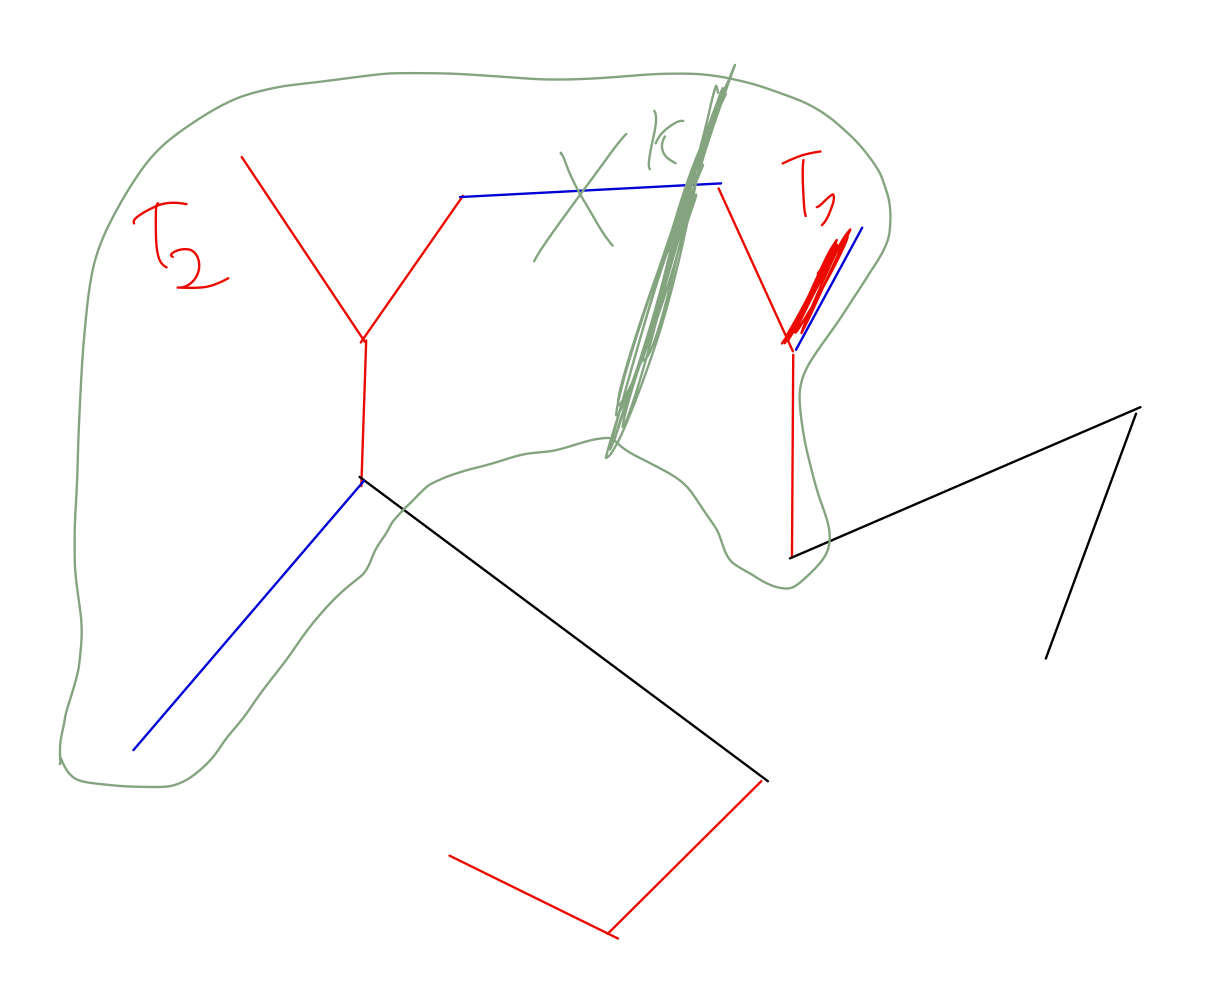
\includegraphics[width=0.5\linewidth]{figures/connectivity_deleting_spanning.jpeg}
	\caption{Deleting an edge.}
	\label{fig:connectivity_deleting_spanning}
\end{figure}

Let's see that all our constraints are satisfied.

We increase level of all edges on tree $T_1$ to make it still appliable when we increase level of new edge from lower level(because we've touched it). Implies that $F_i$ is a maximum spanning tree, implies that $F_i = F_0 \cap G_i$.

Running time:

When we add an edge, we just need to merge two trees. It's being made in time $\log n$.

On deleting an edge we need to make a split on each level, split takes $\log n$, there are no more than $\log n$ levels. And also finding an alternative takes $q \log n$ amortized(because every touched edge is level being upped), to make it we maintain for each tree $T$ all it's edges on level $l$ for every $l$.

Total time is $O(\log^2 n)$ amortized.
\end{proof}

\begin{df}[ET-tree] \label{df:et_tree}
  ET-tree, stores a tree with weights on vertices and allows:
  \begin{enumerate}
	  \item $O(1)$ return sum of weights in entire tree
	\item $O(\log n)$ update weight of a single vertex
	\item $O(\log n)$ to split or merge two ET-trees by given edge
	\item $O(\log n)$ to get a tree in which query vertex belongs to.
	\item $O(\log^2 n)$ Maintains lists of edges on each level, if edges are assigned to levels and maximum level is $O(\log n)$.
  \end{enumerate}
\end{df}

\begin{proof}
	We would store a Euler's route of a tree.
	And also for each vertex we store all pointer to it's position on it's route.

\begin{figure}[H]
	\centering
	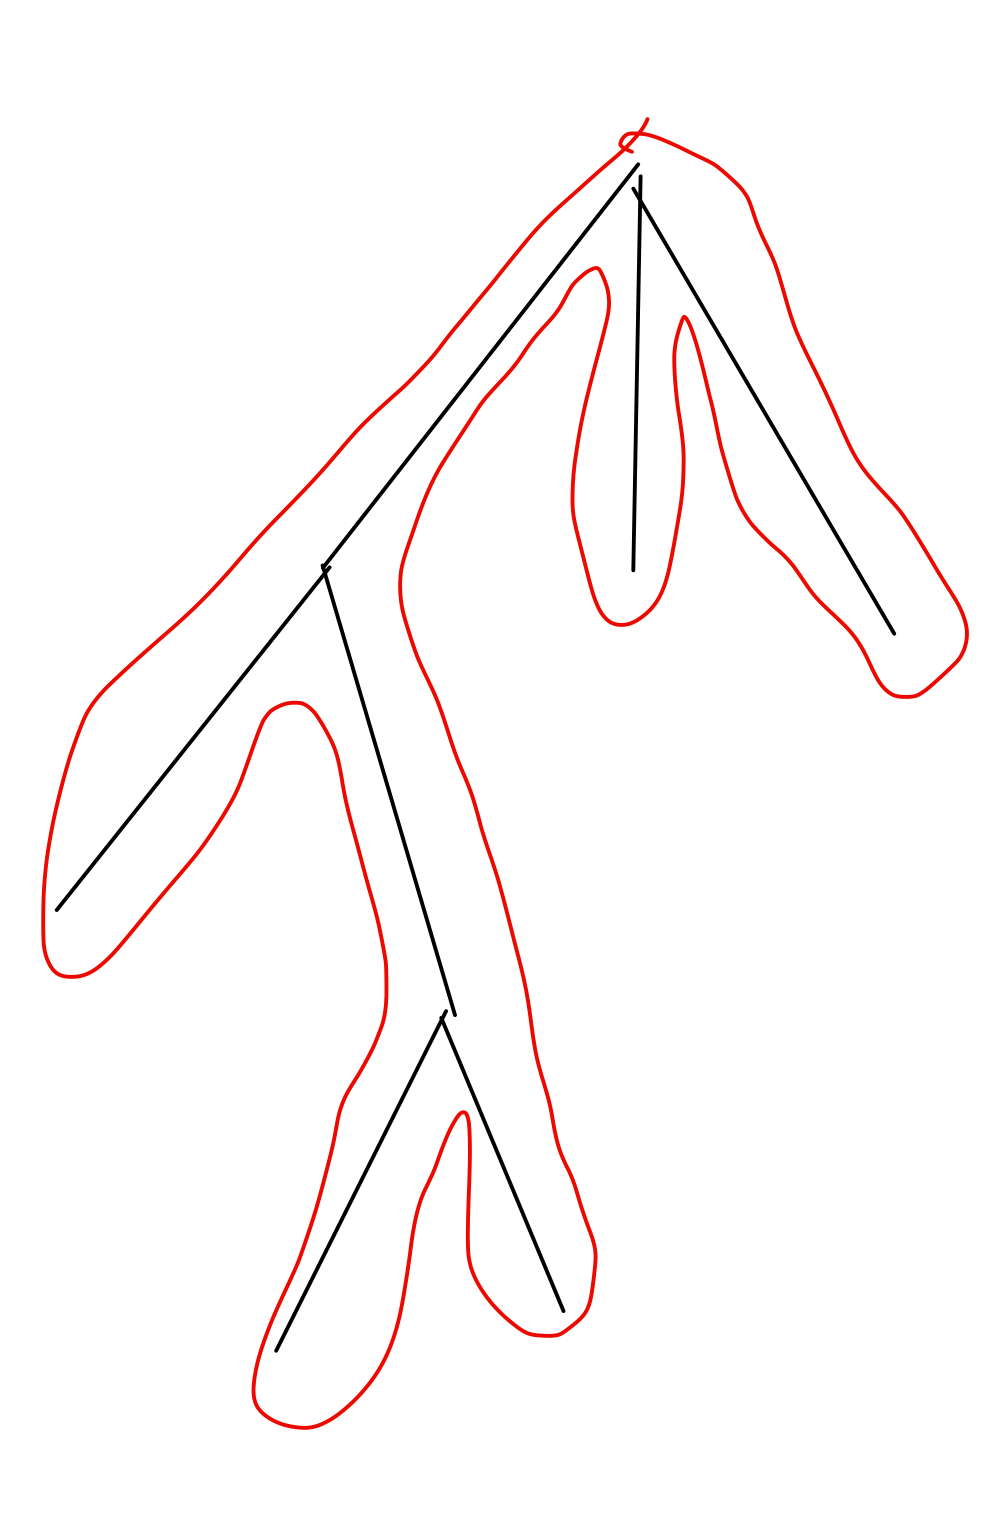
\includegraphics[width=0.3\linewidth]{figures/et_tree_euler.jpeg}
	\caption{Euler's route for a tree.}
	\label{fig:et_tree_euler.jpeg}
\end{figure}

	We store a segment tree of Euler's route, to delete an edge we find it's two positions in route and after that substracting subsegment to a new tree and merge two rest into the second one.
	We do this by using linked-list.
	Same can be done to maintain list of edges on each level.
\begin{figure}[H]
	\centering
	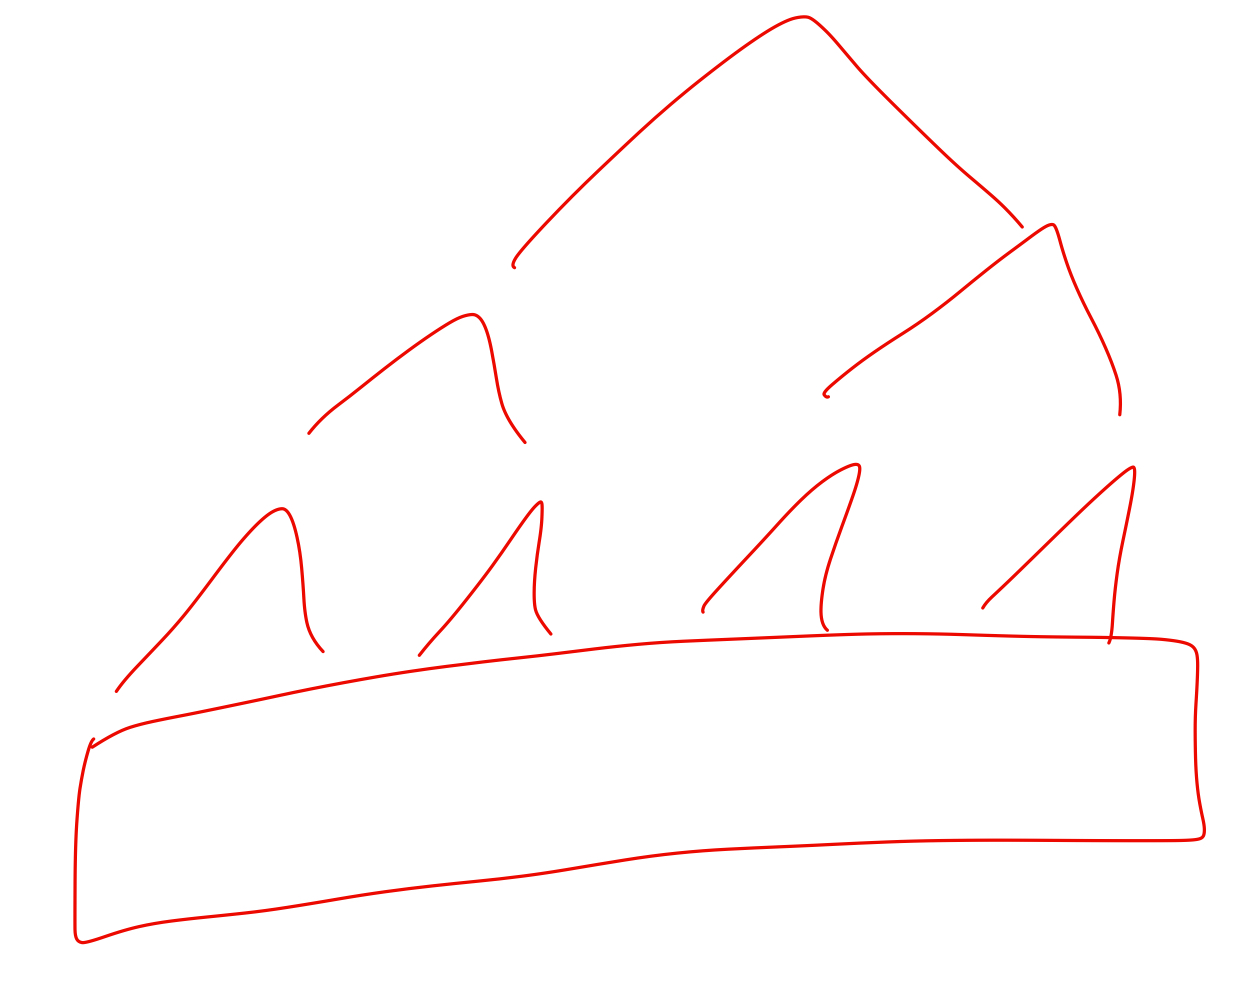
\includegraphics[width=0.3\linewidth]{figures/et_tree_segment_tree.jpeg}
	\caption{Segment tree on Euler's list.}
	\label{fig:et_tree_segment_tree.jpeg}
\end{figure}
\end{proof}

\begin{claim}
  Assume that now firstly we add some edges and at the end we have one query for deleting single edge.

  We can do it with time $O(\log^{O(1)} n)$.
\end{claim}

\begin{proof}[Search-Cut algorithm] \label{algo:search_cut}
	We need to check, whether after deleting an edge, our tree remains connected or not.

Associate each edge $e = \{v_i, v_j\}$ with a number $l(e) = i \circ j$.

  Then, 
  \begin{align}
	  \bigoplus_{v \in T_1} \bigoplus_{u \colon (v, u) \in E} l(\{v, u\}) \label{eq:connectivity_xor}
  \end{align} is just a xor of all edges from $T_1$ to $T_2$, means that if there is a single alternative of $e$, then we would find it immediately.
  Then, using our ET-tree \ref{df:et_tree} putting weight of a vertice to be equal to xor of all it's adjacent edges we can do it fast.

  We would make approximately $\log n$ "substreams"(same as in Sparse Recovery).
  In a first substream we would take each edge with probability 1, in second with $\frac{1}{2}$, in third with $\frac{1}{4}$ and so on.
  Then, with constant probability there would be a single edge on some level that connectes $T_1, T_2$.

  In Eq. \eqref{eq:connectivity_xor} it's value or equal to some correct edge, or some trash. And we can check it.

\end{proof}

\begin{remrk}
  And we cannot easily make it to delete many edges, because we need to reconstruct our sample levels to make them independent.
\end{remrk}

\begin{claim}
  To make it work, we use algorithm Boruvki.

  It's iterative. Firsly, it constructs spanning tree of size 1, then of size 2, and so on.

  Also we would use algorithm SearchCut \ref{algo:search_cut} that would find an edge that goes outside of a tree with constant probability. 

  Wanted property: if for tree $T$ SearchCut gives outside vertex, then on next level we would merge this tree to someone.

  It gives us that on every level amount of components decreases exponentially.

  \begin{figure}[H]
  	\centering
  	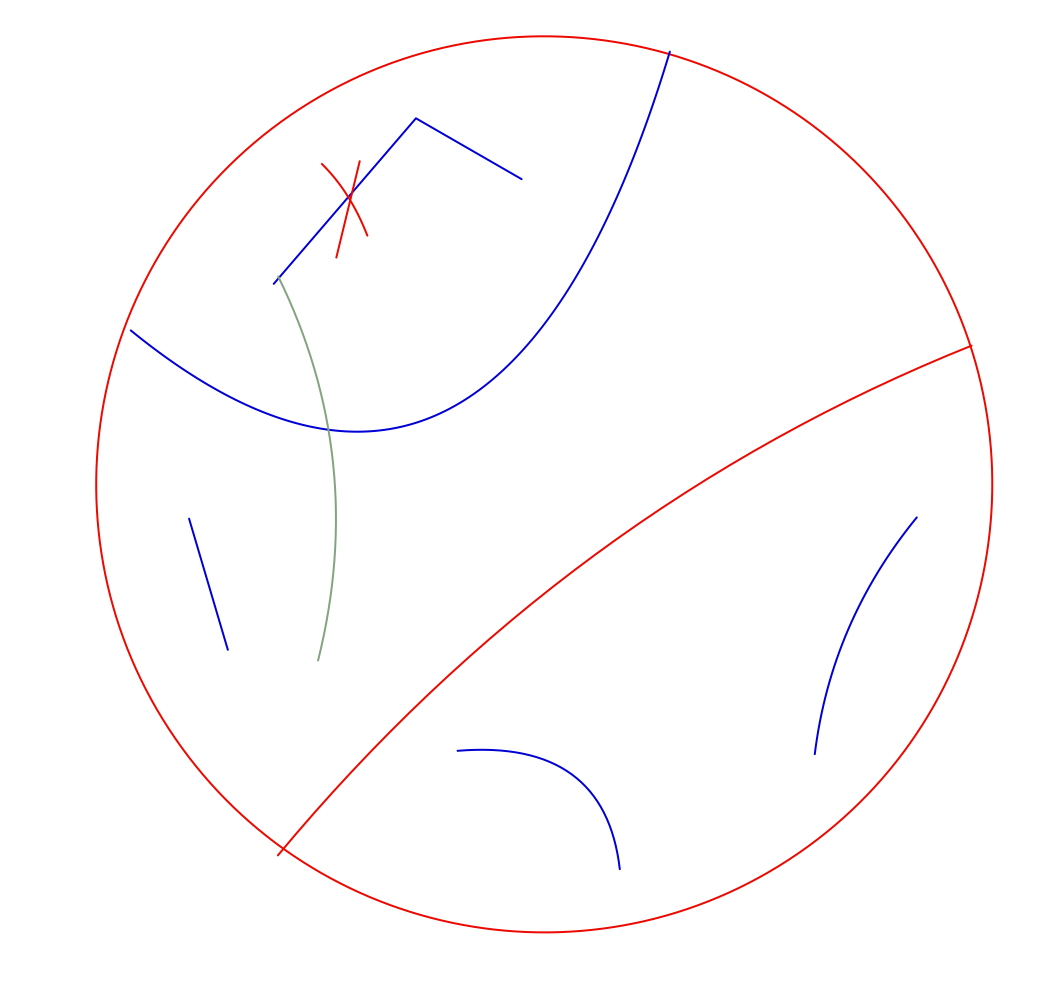
\includegraphics[width=0.5\linewidth]{figures/boruvka_search_cut.jpeg}
  	\caption{Something with boruvka and search cut...}
  	\label{fig:boruvka_search_cut}
  \end{figure}
\end{claim}
